When the numerical analysis results produced on the cb-2 via the CodeMR tool are reviewed, it is seen that the tool analyzes 1160 lines of code belonging to this codebase. These lines of code belong to 139 classes in 59 different packages of 4 different features which were mentioned in section \ref{section:4.3.1}. When the CodeMR analysis results of this codebase are examined, a very positive situation is encountered. In the figure below, a CodeMR table that reflects the general situation of cb-2 is shared.
\begin{figure}[ht!]
    \centering
    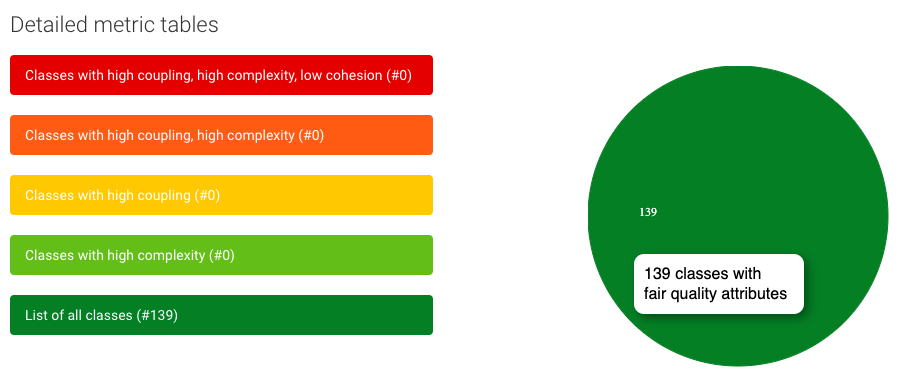
\includegraphics[scale=0.45]{figures/cb-2-metric-table.png}
    \caption{CodeMR Metrics Overview of CB-2}
    \label{fig:cb-2-metric-table.png}
\end{figure}
\FloatBarrier

Between the analyzed classes, it is seen that two classes corresponding to 9\% of the total code size have low-medium WMC values, and the rest of the classes appear to have a low level of WMC values. It appears that the majority of the classes belong to cb-2 have low complexity levels. When the values of the DIT metric of the classes are examined, it is seen that 10 classes, corresponding to 28.9\% of the total code size, have middle-upper level DIT values and the other 27 classes corresponding to 14.1\% of the total code size have low-medium level DIT values. The rest of the classes have a low level of DIT values.  When DIT values of these classes are examined, it is seen that some classes have a DIT value of 2 and classes with more than a DIT value of 2 values are quite low (DIT values between 1-3 considered as low-medium by CodeMR). When the NOC metric values of the classes are examined, it is seen that 7 classes corresponding to only 6.6\% of the whole codebase have low-medium NOC values, and 1 very concise class has medium-high NOC value. The rest of the classes have low NOC values. According to the results, it is seen that ten classes are corresponding to 26.6\% of the application's code volume with a low-medium COB value and the rest of the classes have a low COB value. According to the results of the CodeMR analysis, all classes within the cb-2 have low LCOM values. According to the results of the CodeMR analysis, all classes within the cb-2 have low LCOM values. In the figure below, the results of the class-based metric values, which is detailed and interpreted above, visualized by the "Metric Distribution" method offered by the CodeMR tool are presented.

\begin{figure}[ht!]
    \centering
    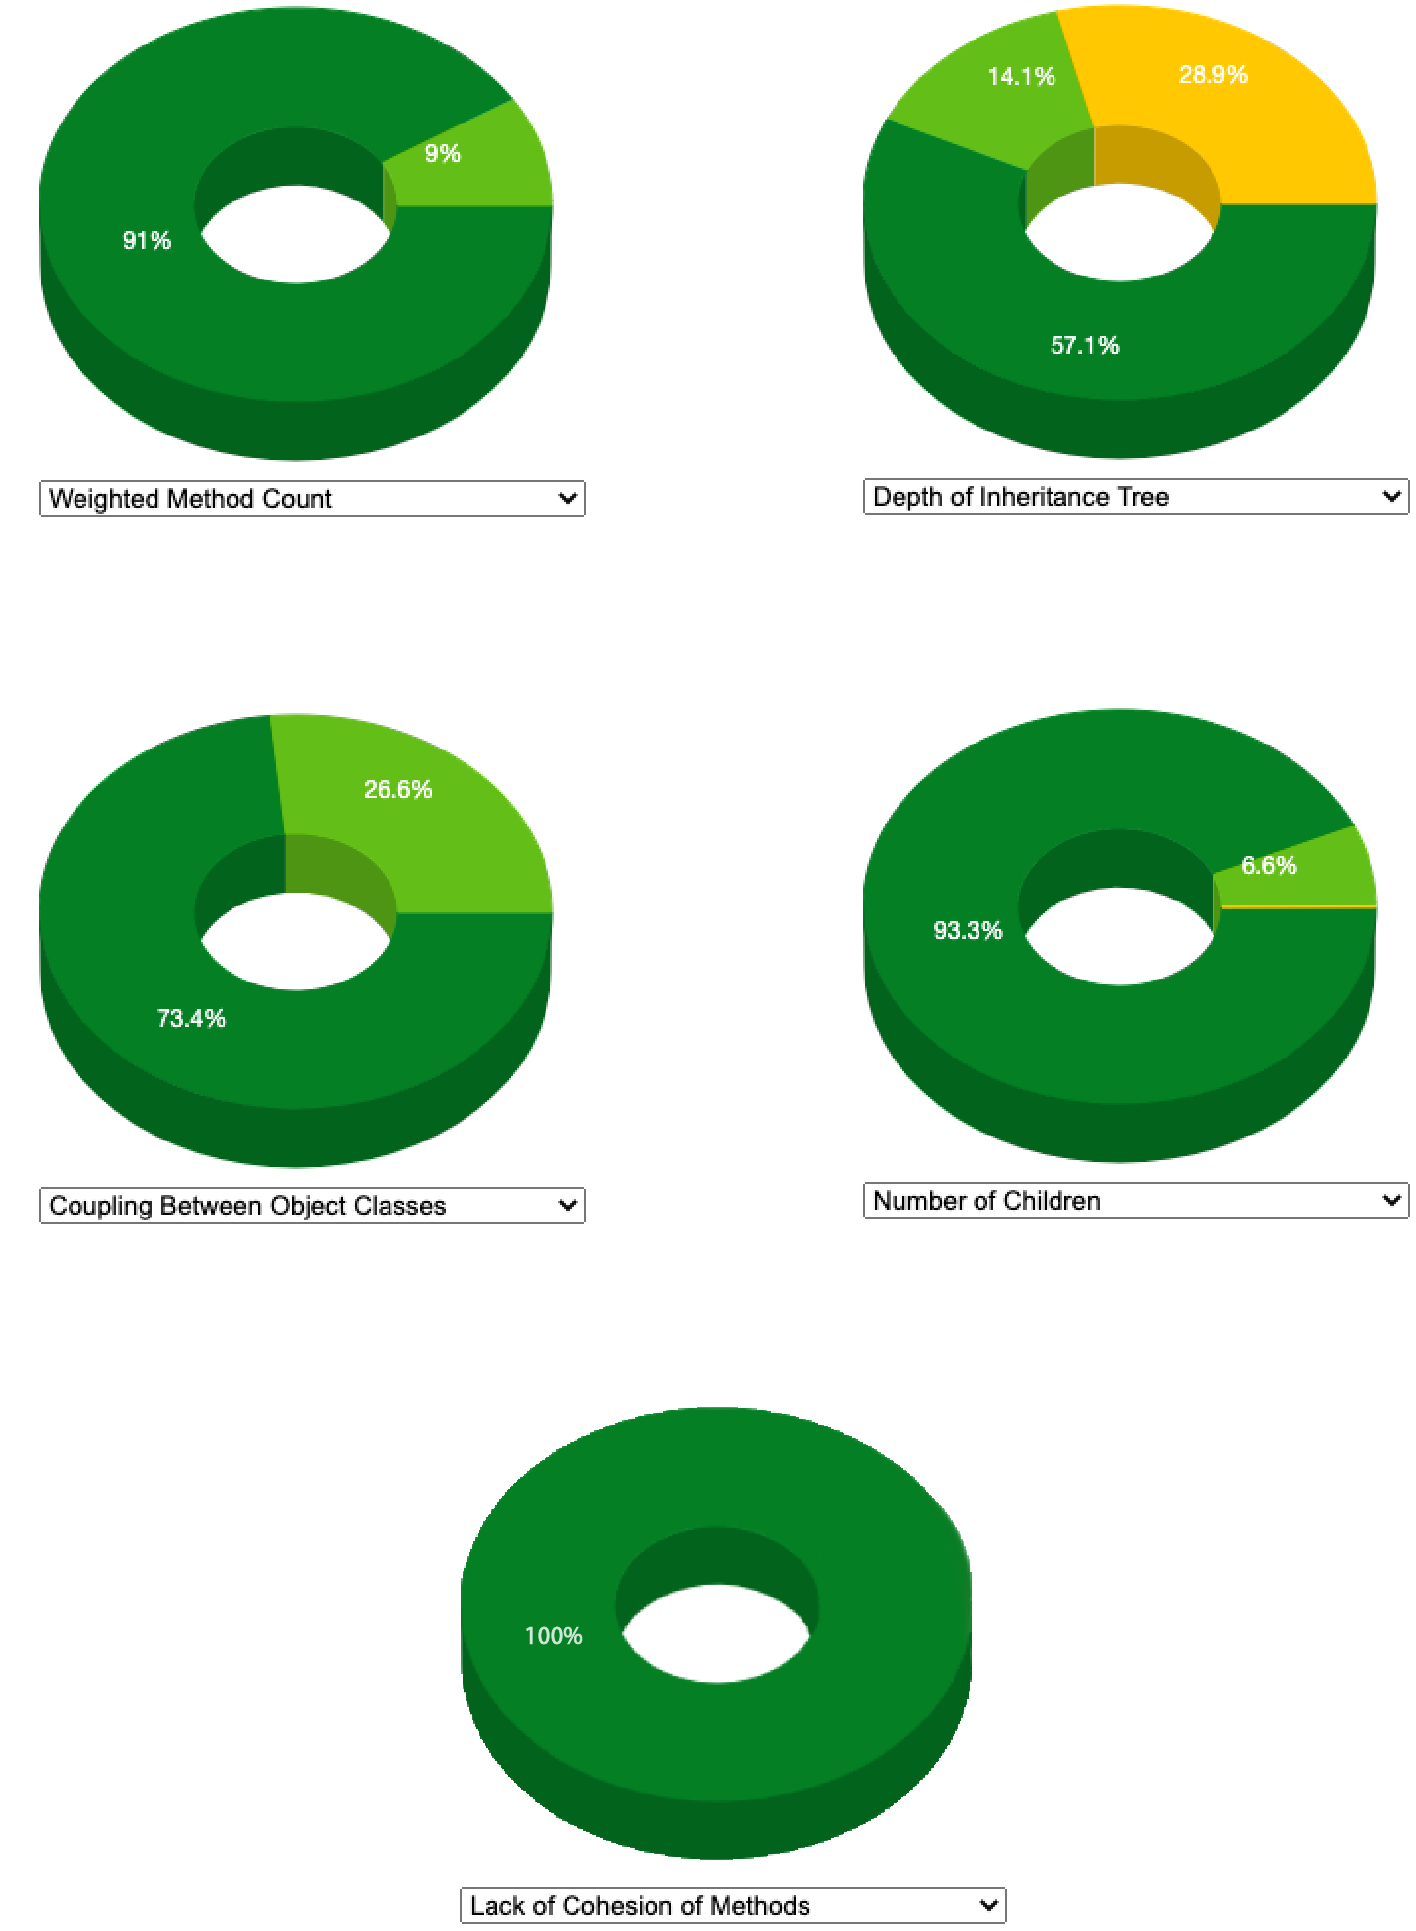
\includegraphics[scale=1]{figures/cb-2-donuts.png}
    \caption{CodeMR Metric Distribution for CB-2}
    \label{fig:cb-2-donuts}
\end{figure}
\FloatBarrier

In the figure below, a general view of cb-2 in terms of complexity, coupling and cohesion is shown. As explained in the previous section, the largest circle represents the project, inner circles represent the packages and small circles inside the inner circles represent the classes. Sizes of the circles proportional to the size of the represented entity.
\begin{figure}[ht!]
    \centering
    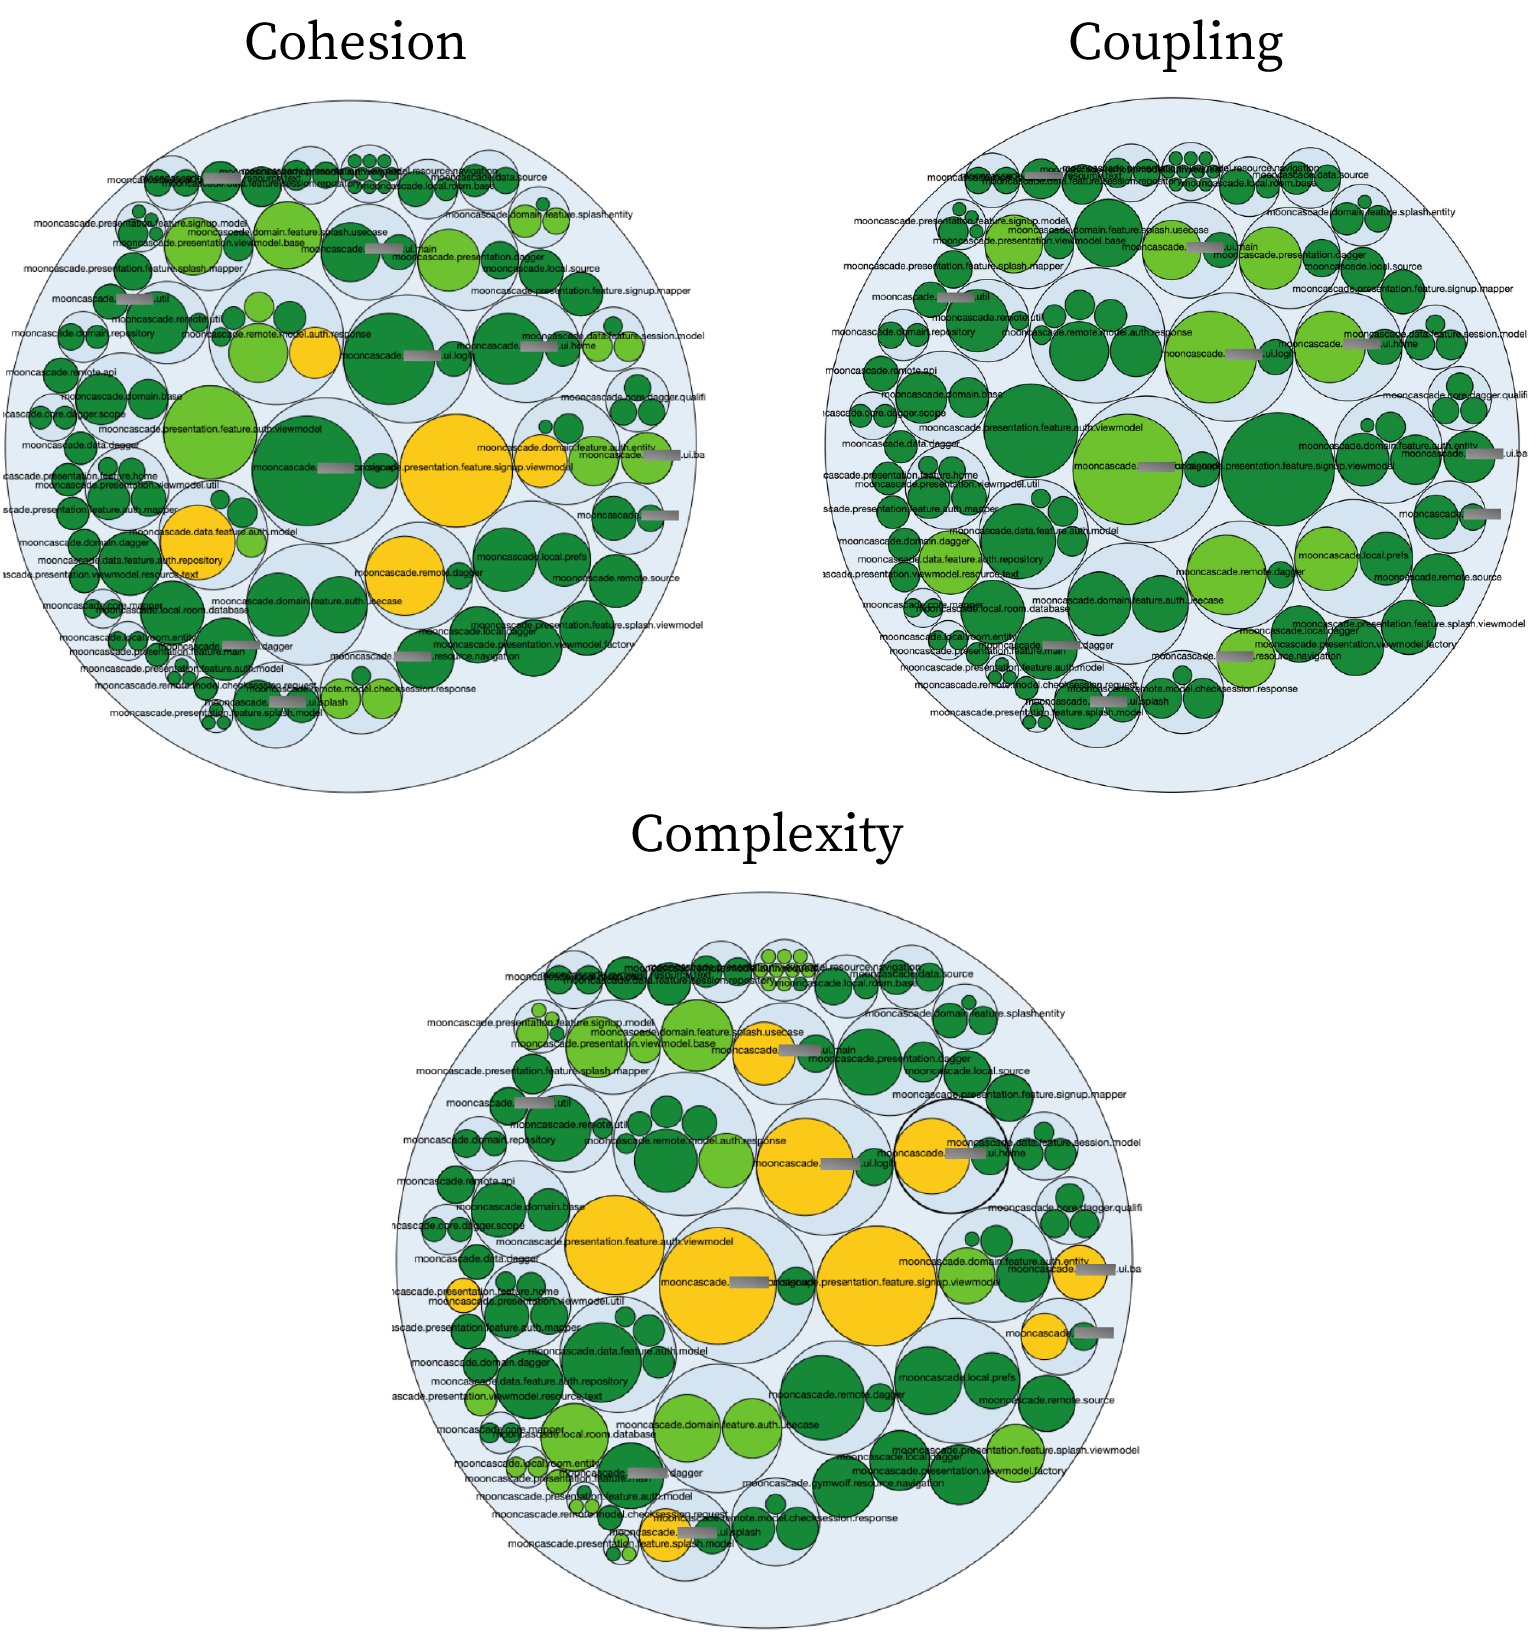
\includegraphics[scale=1.1]{figures/cb-2-package.png}
    \caption{CodeMR Metric Distribution for CB-2}
    \label{fig:cb-2-package}
\end{figure}
\FloatBarrier





